\begin{frame}{Erkennung des Queues}
\textbf{Problem:} Damit der Spieler die Kugeln mit dem Queue spielen kann, muss dieser im Kamerabild erkannt werden

\pause

\textbf{Unsere Lösung}:
\begin{itemize}
	\item[1.] Queue vom Hintergrund des Bildes segmentieren\\
	\pause
	$\implies$ zur Vereinfachung ist der Queue schwarz gefärbt
	\pause
	\item[2.] Hauptachse des Queues bestimmen
	\pause
	\item[3.] Durch die Hauptachse die beiden Endpunkte des Queues bestimmen
	\pause
	\item[4.] Die Endpunkte in Spielkoordinaten transformieren
	\pause
	\item[5.] Mit \textbf{beiden} Endpunkten die übliche Kollision ausführen
	
\end{itemize}
\end{frame}

\begin{frame}{Erkennung des Queues: Lösung}
\begin{itemize}
	\item [1.] Queue vom Hintergrund des Bildes segmentieren:
\end{itemize}
\begin{center}
\visible<1->{\stackunder[5pt]{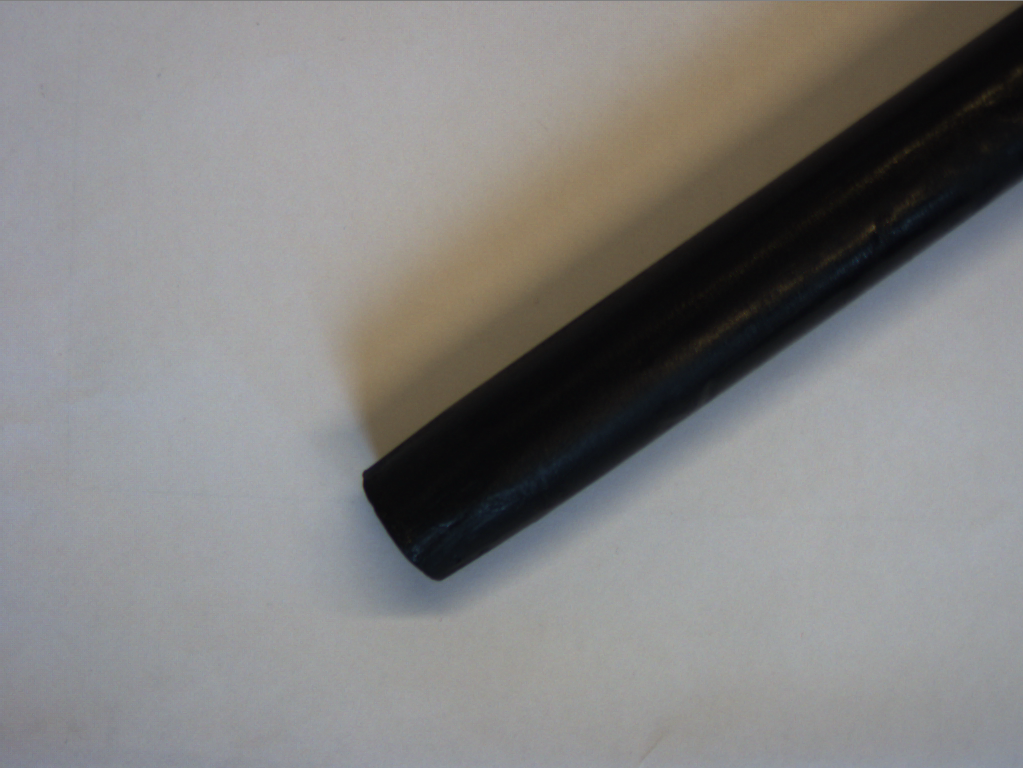
\includegraphics[height=2.3cm]{bilder/queue_orig.png}}{Kamerabild}}
\visible<2->{\stackunder[5pt]{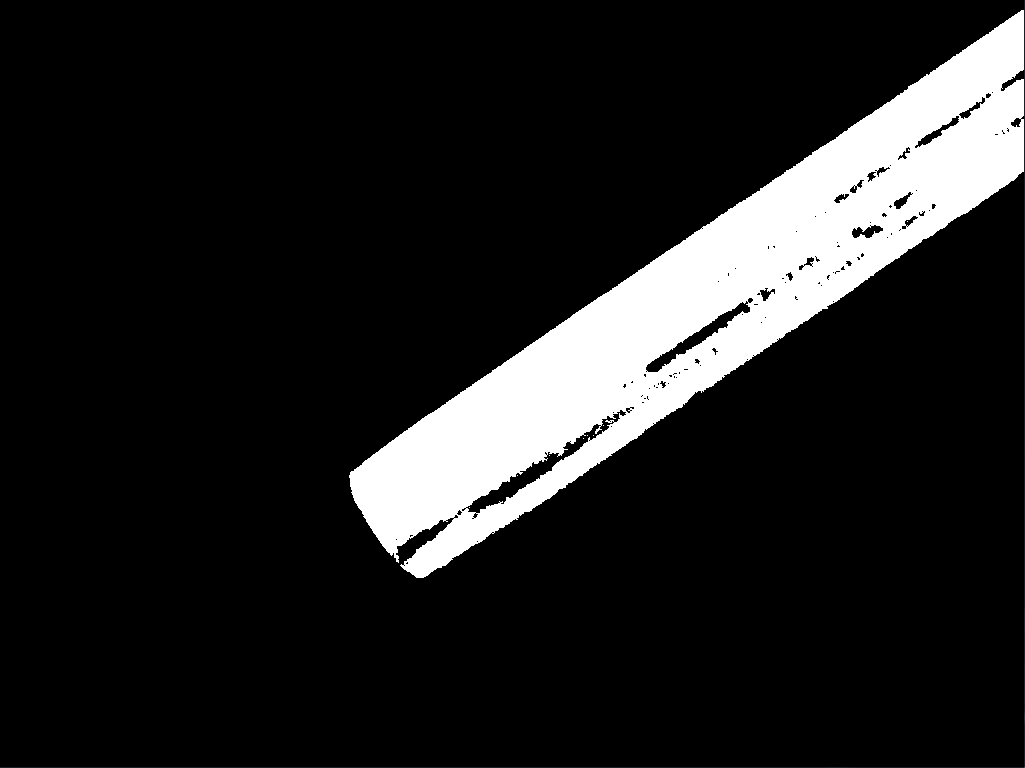
\includegraphics[height=2.3cm]{bilder/queue_thresholded.png}}{Segmentierung}}
\visible<3->{\stackunder[5pt]{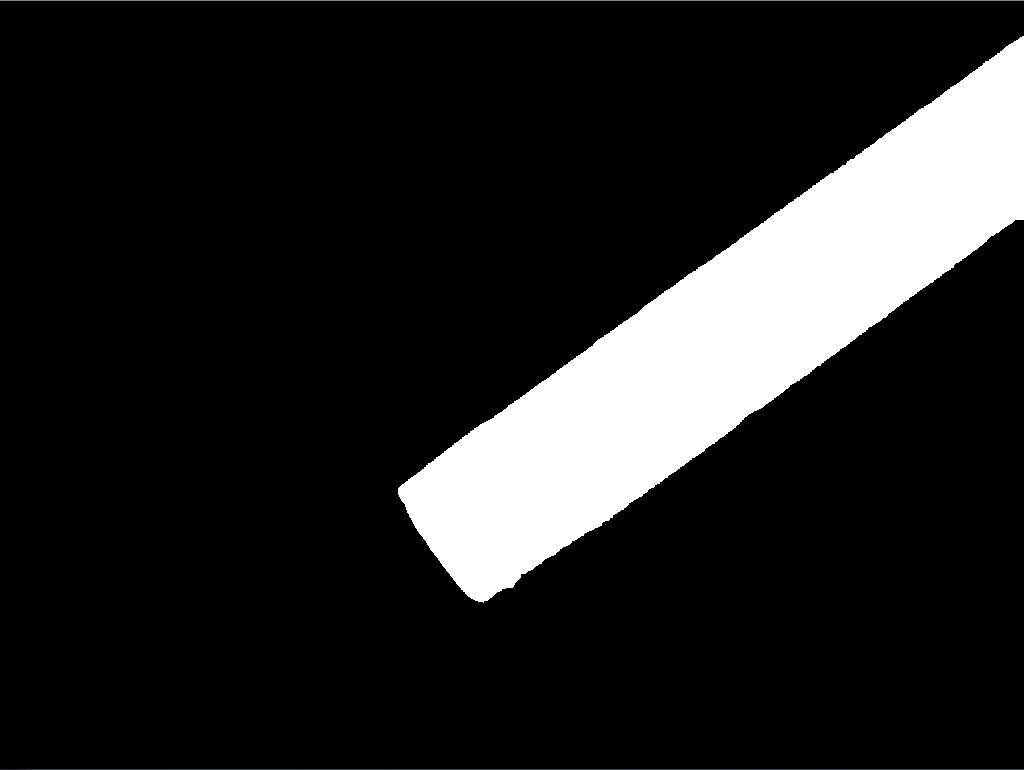
\includegraphics[height=2.3cm]{bilder/queue_close.png}}{Closing}}
\end{center}
\end{frame}
\begin{frame}{Kollision mit Queue: Lösung}
\begin{itemize}
	\item [2.] Hauptachse des Queues bestimmen\\
	$\implies$ durch Hauptkomponentenanalyse (PCA)
	
	\item [3.] Durch die Hauptachse die beiden Endpunkte des Queues bestimmen
\end{itemize}
\begin{center}
	\visible<1->{\stackunder[5pt]{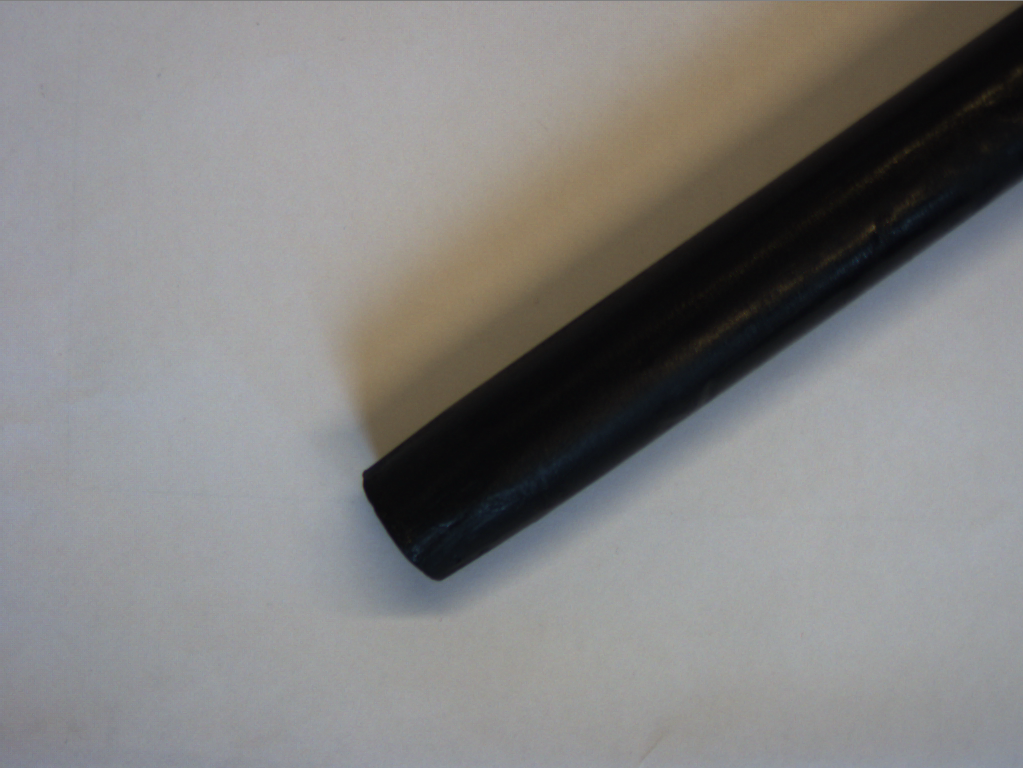
\includegraphics[height=2.3cm]{bilder/queue_orig.png}}{Kamerabild}}
	\visible<2->{\stackunder[5pt]{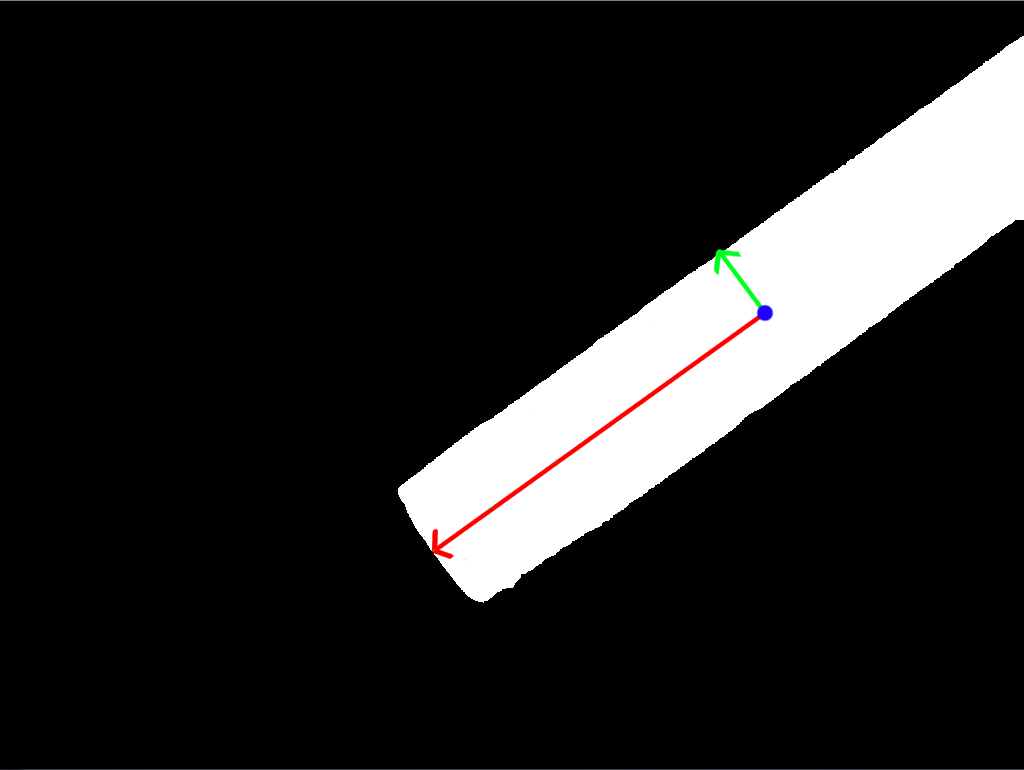
\includegraphics[height=2.3cm]{bilder/queue_pca_1.png}}{Ergebnis PCA}}
	\visible<3->{\stackunder[5pt]{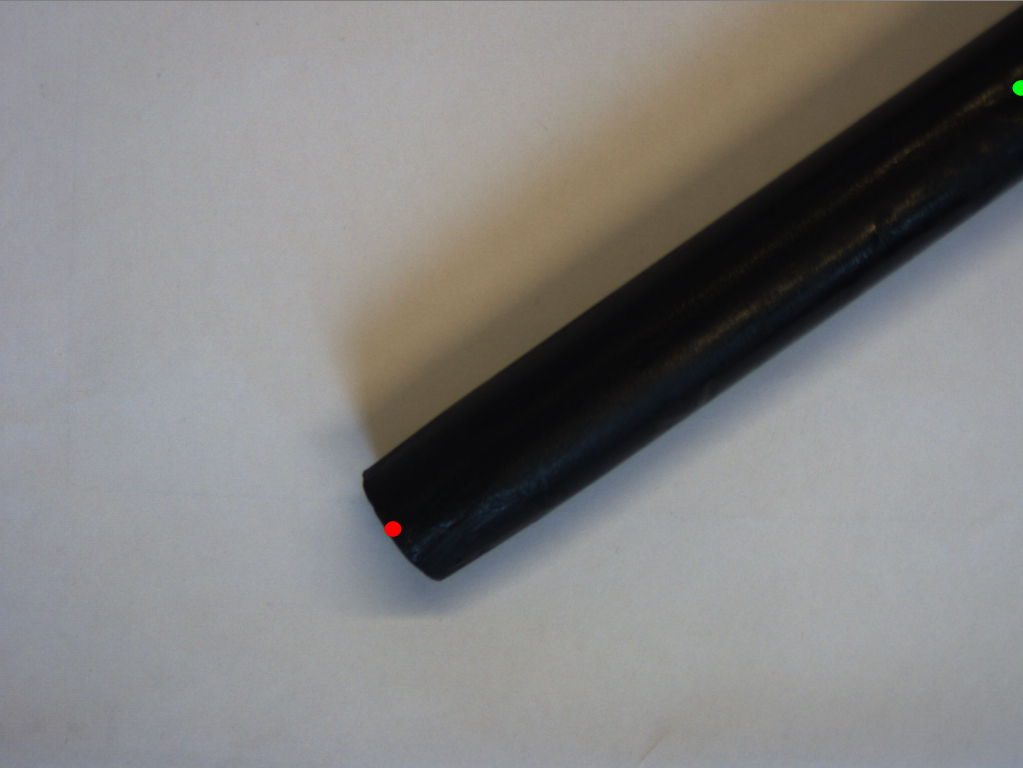
\includegraphics[height=2.3cm]{bilder/queue_pca_2.png}}{Bestimmte Endpunkte}}
\end{center}
\end{frame}

\begin{frame}{Erkennung des Queues: Lösung}
\begin{itemize}
	\item[4.] Die Endpunkte in Spielkoordinaten transformieren
	\item [5.] Mit den Endpunkten übliche Kollision ausführen	
\end{itemize}
\pause
\textbf{Problem:} Aufnahmen nur mit 24 Bildern pro Sekunde möglich\\
$\implies$ Kollisionen bei schneller Bewegung wird eventuell nicht erkannt!
\pause
\textbf{Lösung:}  Berechnung des Kollisionspunktes durch Interpolation
\begin{center}
	\visible<4->{\stackunder[5pt]{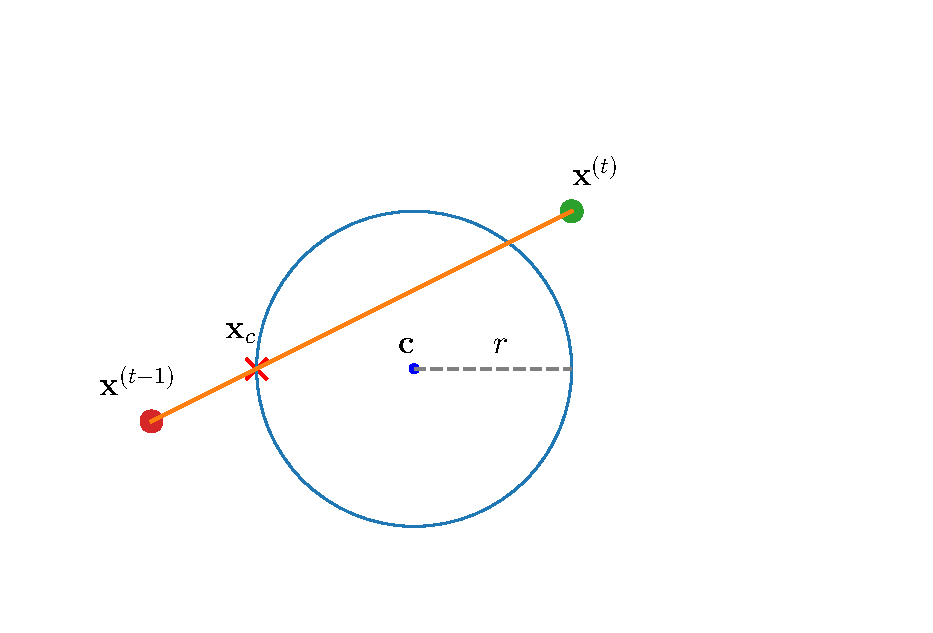
\includegraphics[height=2.7cm]{bilder/hit.eps}}{Kollision}}
	\visible<5->{\hspace{-0.7cm}\stackunder[5pt]{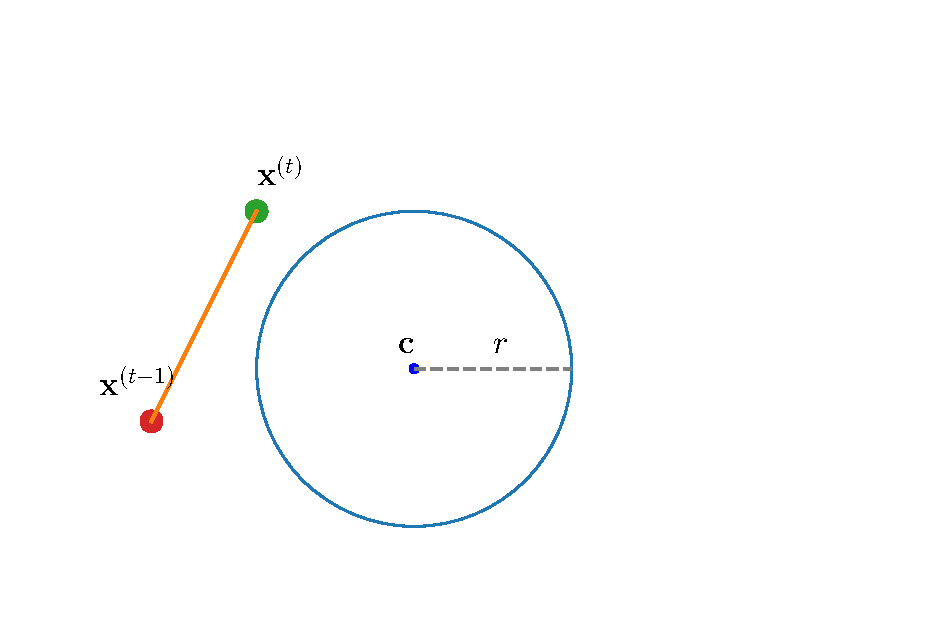
\includegraphics[height=2.7cm]{bilder/nohit.eps}}{Keine Kollision}}
	\visible<6->{\hspace{-1.2cm}\stackunder[5pt]{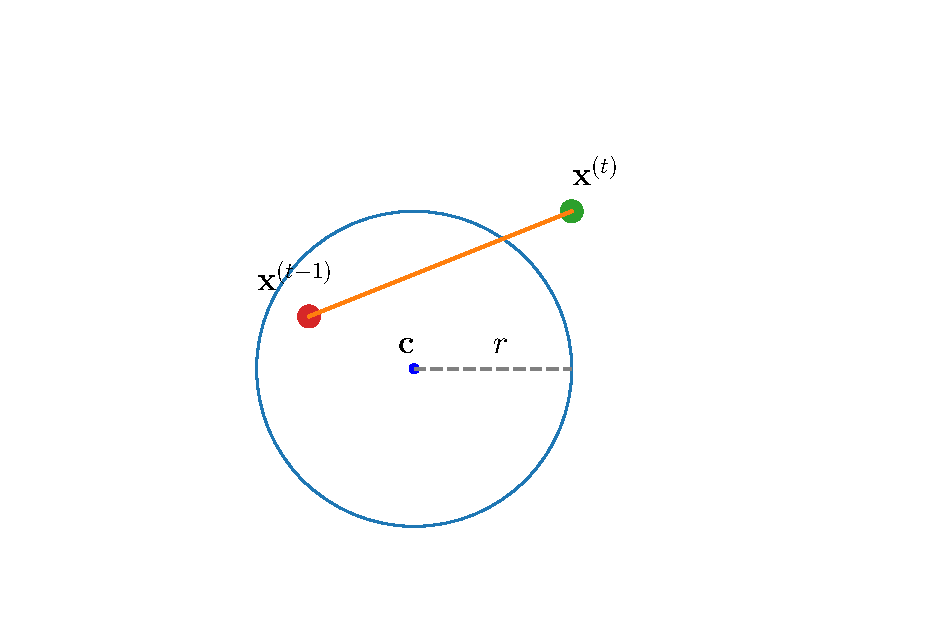
\includegraphics[height=2.7cm]{bilder/exitwound.eps}}{Keine Kollision}}
\end{center}
\end{frame}
\begin{frame}{Erkennung des Queues: Fazit}
	Die vorgestellte Lösung würde sich noch verbessern lassen:
	\begin{itemize}
		\pause
		\item Segmentierung  (und damit alle folgenden Schritte) stark von der Umgebung abhängig\\
		$\implies$ Verbesserung z.B. durch markerbasierte Erkennung
		\pause
		\item Wiederholfrequenz/Belichtungszeit der Kamera verursacht Bewegungsunschärfe\\
		$\implies$ Ungenauigkeit der Erkennung
	\end{itemize}
\end{frame}


